\documentclass[spanish,a4paper,14pt,oneside]{extreport}

\usepackage[utf8]{inputenc}
\usepackage[spanish]{babel}
\usepackage[pdftex]{graphicx}
\usepackage{hyperref}
\usepackage{url}
\graphicspath{{Imagenes/}}
\usepackage{listings}
\usepackage{color}

%\usepackage{biblatex}
%\usepackage[dvips]{graphicx}
%\usepackage[dvips]{epsfig}
%\usepackage{alltt}
%\usepackage{algorithm}
%\usepackage{algorithmic}
%\usepackage{multirow}
%\usepackage[top=2cm, bottom=2cm, left=2cm, right=2cm]{geometry}

%Evitar partir palabras al final de la línea
\hyphenpenalty=10000
\tolerance=1000

%%%%%%%%%%%%%%ESTILO PARA CÓDIGO%%%%%%%%%%%%%%%%%%%%%%%%%%%%%%%%%%%%%%%
\definecolor{violet}{rgb}{0.5,0,0.5}
\definecolor{navy}{rgb}{0,0,0.5}
\definecolor{hellgelb}{rgb}{0.95,0.95,0.92}
\definecolor{colKeys}{rgb}{0,0,1}
\definecolor{colIdentifier}{rgb}{0,0,0}
\definecolor{colComments}{rgb}{1,0,0}
\definecolor{colString}{rgb}{0,0.5,0}

\lstset{
	float=htbp,
	language = Java,
	basicstyle=\ttfamily\small,
	identifierstyle=\color{colIdentifier},
	keywordstyle=\color{colKeys},
	stringstyle=\color{colString},
	commentstyle=\color{colComments},
	columns=flexible,
	tabsize=3,
	frame=single,
	extendedchars=true,
	showspaces=false,
	showstringspaces=false,
	numbers=left,
	numberstyle=\tiny,
	breaklines=true,
	backgroundcolor=\color{hellgelb},
	breakautoindent=true,
	captionpos=b,
	breakatwhitespace=true,
	aboveskip=10pt,
	belowskip=10pt,
}

\renewcommand{\lstlistingname}{Listado} % Los títulos de los códigos insertados se denotan con Listado...
%\renewcommand{\lstlistingname}{Ejemplo} % Los títulos de los códigos insertados se denotan con Ejemplo...

%%%%%%%%%%%%%%%%%%%%%%%%%%%%%%%%%%%%%%%%%%%%%%%%%%%%%%%%%%%%%%%%%%%%%%%%%%%%%%%%%%%%%%%%%%%%%%%%
\newcommand{\CollegeApp}{\texttt{SchoolApp }{}}
\newcommand{\workTitle}{\texttt{``SchoolApp'': Comunicación desde las aulas.}{}}
\newcommand{\englishWorkTitle}{\texttt{``SchoolApp'': Comunication from the classroom.}{}}

\newenvironment{summary}{
	\par
	\noindent
	\begin{center}
		\textbf{Abstract}
	\end{center}
	\begin{itshape}
		\par
		\noindent
	\end{itshape}}

%%%%%%%%%%%%%%%%%%%%%%%%%%%%%%%%%%%%%%%%%%%%%%%%%%%%%%%%%%%%%%%%%%%%%%%%%%%%%%%%%%%%%%%%%%%%%%%%

\begin{document}
	%%%%%%Capitulos definitivos%%%%%%
	%
% ---------------------------------------------------
%
% Trabajo de Final de Grado:
% Author: Gonzalo Jesús García Martín <dracoyue@gmail.com>
% Capítulo: Portada
% Fichero: Portada.tex
%
% ----------------------------------------------------
%

\pagestyle{empty}
\thispagestyle{empty}


\newcommand{\HRule}{\rule{\linewidth}{1mm}}
\setlength{\parindent}{0mm}
\setlength{\parskip}{0mm}

\vspace*{\stretch{0.5}}

\begin{center}

\includegraphics[scale=0.8]{Imagenes/logo_vertical}\\[10mm]
{\Huge Trabajo de Fin de Grado}
\end{center}

\HRule
\begin{flushright}
        {\Huge Título} \\[2.5mm]
        {\Large \textit{Title in English} .} \\[5mm]
        {\Large Gonzalo J. García Martín} \\[5mm]


\end{flushright}
\HRule
\vspace*{\stretch{2}}
\begin{center}
  \Large La Laguna, \today
\end{center}

\setlength{\parindent}{5mm} %Listo
	%
% ---------------------------------------------------
%
% Trabajo de Final de Grado:
% Author: Gonzalo Jesús García Martín <dracoyue@gmail.com>
% Capítulo: Certificado
% Fichero: Certificado.tex
%
% ----------------------------------------------------
%

\newpage
%\cleardoublepage
\thispagestyle{empty}

D. {\bf Francisco de Sande González}, con DNI número 42067050--G
profesor Titular de Universidad adscrito al Departamento de Ingeniería Informática y de Sistemas
de la Universidad de La Laguna, como tutor

\bigskip
\bigskip
{\bf C E R T I F I C A}

\bigskip
\bigskip
\bigskip
Que la presente memoria titulada:

\bigskip
``{\it Título del Trabajo.}''

\bigskip
\bigskip
\bigskip

\noindent ha sido realizada bajo su dirección por D. {\bf Gonzalo J. García Martín},
con N.I.F. 78.628.877-K.

\bigskip
\bigskip

Y para que así conste, en cumplimiento de la legislación vigente y a los efectos
oportunos firman la presente en La Laguna a \today

%\cleardoublepage
%\newpage
 %Listo
	%
% ---------------------------------------------------
%
% Trabajo de Final de Grado:
% Author: Gonzalo Jesús García Martín <dracoyue@gmail.com>
% Capítulo: Agradecimientos
% Fichero: Agradecimientos.tex
%
% ----------------------------------------------------
%

\thispagestyle{empty}

{\flushright

	\begin{LARGE}
		Agradecimientos
	\end{LARGE}

	\hspace{3mm}

	\begin{large}

		\hspace{3mm}
		XXX
	
		\hspace{3mm}
		XXX
	
		\hspace{3mm}
		XXX
	
		\hspace{3mm}
		XXX

	\end{large}

} %Listo
	\newpage

\begin{huge}
Licencia
\end{huge}

\bigskip
* Si NO quiere permitir que se compartan las adaptaciones de tu obra
y NO quieres permitir usos comerciales de tu obra indica:

\begin{center}
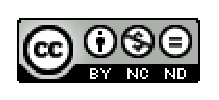
\includegraphics[scale=1.5]{Imagenes/Licencias/by-nc-nd_88x31}\\[10mm]
{\Large \copyright~Esta obra está bajo una licencia de Creative Commons Reconocimiento-NoComercial-SinObraDerivada 4.0 Internacional.
}
\end{center}


\bigskip
* Si quiere permitir que se compartan las adaptaciones de tu obra mientras se comparta de la misma manera
y NO quieres permitir usos comerciales de tu obra indica:

\begin{center}

\includegraphics[scale=1.5]{Imagenes/Licencias/by-nc-sa_88x31}\\[10mm]
{\Large \copyright~Esta obra está bajo una licencia de Creative Commons Reconocimiento-NoComercial-CompartirIgual 4.0 Internacional.
}
\end{center}



\bigskip
* Si quiere permitir que se compartan las adaptaciones de tu obra
y NO quieres permitir usos comerciales de tu obra indica:

\begin{center}

\includegraphics[scale=1.5]{Imagenes/Licencias/by-nc_88x31}\\[10mm]
{\Large \copyright~Esta obra está bajo una licencia de Creative Commons Reconocimiento-NoComercial 4.0 Internacional.
}
\end{center}

\newpage

\bigskip
*Si NO quiere permitir que se compartan las adaptaciones de tu obra
y quieres permitir usos comerciales de tu obra indica:

\begin{center}
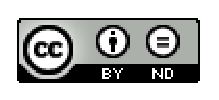
\includegraphics[scale=1.5]{Imagenes/Licencias/by-nd_88x31}\\[10mm]
{\Large \copyright~Esta obra está bajo una licencia de Creative Commons Reconocimiento-SinObraDerivada 4.0 Internacional.
}
\end{center}


\bigskip
* Si quiere permitir que se compartan las adaptaciones de tu obra mientras se comparta de la misma manera
y quieres permitir usos comerciales de tu obra (licencia de Cultura Libre) indica:

\begin{center}

\includegraphics[scale=1.5]{Imagenes/Licencias/by-sa_88x31}\\[10mm]
{\Large \copyright~Esta obra está bajo una licencia de Creative Commons Reconocimiento-CompartirIgual 4.0 Internacional.
}
\end{center}


\bigskip
* Si quiere permitir que se compartan las adaptaciones de tu obra
y quieres permitir usos comerciales de tu obra (licencia de Cultura Libre) indica:

\begin{center}

\includegraphics[scale=1.5]{Imagenes/Licencias/by_88x31}\\[10mm]
{\Large \copyright~Esta obra está bajo una licencia de Creative Commons Reconocimiento 4.0 Internacional.
}
\end{center}
 %Listo
	%
% ---------------------------------------------------
%
% Trabajo de Final de Grado:
% Author: Gonzalo Jesús García Martín <dracoyue@gmail.com>
% Capítulo: Resumen
% Fichero: Resumen.tex
%
% ----------------------------------------------------
%

\newpage  %\cleardoublepage
\begin{abstract}
	{\em
		%\bigskip
		El objetivo general de este proyecto ha sido crear una aplicación para \textit{Android} usando las nuevas tecnologías y los servicios de almacenamiento en internet, comúnmente conocidos como nube. Se pretende establecer un sistema de comunicación escolar para que los padres, madres, tutores legales, profesores y alumnos estén comunicados entre sí, intentando suplir una carencia en las aulas.
	}
\end{abstract} %Listo
	%
% ---------------------------------------------------
%
% Trabajo de Final de Grado:
% Author: Gonzalo Jesús García Martín <dracoyue@gmail.com>
% Capítulo: Summary
% Fichero: Summary.tex
%
% ----------------------------------------------------
%

\newpage  %\cleardoublepage
\begin{summary}
	{\em
		%\bigskip
		The overall objective of this project was to create an \textit{Android} application using new technologies and the Internet storage services, commonly known as cloud. It was intended to establish a system of school communication for parents, guardians, teachers and students are interconnected.
		
		\bigskip
		With the use of these technologies has increased the number of school problems. It's not just those originating inside the classrooms and teachers can control, but also they have spread to affect students in other areas.
		
		\bigskip
		On this basis, and with the knowledge acquired throughout the Degree in Computer Engineering from the University of La Laguna, it has designed an application that can assist in academia.
		
		\bigskip
		For this we used the integrated development environment, AndroidStudio, along with Firebase, a provider of cloud services.
		
		\bigskip
		{\bf Keywords:} Android applications, mobile devices, schools, education, communication tools.
	}
\end{summary}
 %Listo
	
	%%%%%%%%%%Numeracion en romanos%%%%%%%%%%
	\renewcommand{\thepage}{\roman{page}}
	\setcounter{page}{1}
	%%%%%%%%%%%%%%%%%%%%%%%%%%%%%%%%%%%%%%%%%
	
	%Índices
	\tableofcontents
	\newpage{\pagestyle{empty}}
	\listoffigures
	\newpage{\pagestyle{empty}}
	%\listoftables
	%\newpage{\pagestyle{empty}}
	\renewcommand{\lstlistlistingname}{Índice de Códigos} % Para que no aparezca listings
	\lstlistoflistings
	\newpage{\pagestyle{empty}}
	
	%%%Numeracion a partir del capitulo 1%%%%
	\renewcommand{\thepage}{\arabic{page}}
	\setcounter{page}{1}
	%%%%%%%%%%%%%%%%%%%%%%%%%%%%%%%%%%%%%%%%%
	
	%
% ---------------------------------------------------
%
% Trabajo de Final de Grado:
% Author: Gonzalo Jesús García Martín <dracoyue@gmail.com>
% Capítulo: Introducción
% Fichero: Cap1_Introduccion.tex
%
% ----------------------------------------------------
%

\cleardoublepage
\chapter{Introducción}
\label{chap:intorduction}

%¿Cúal es el tema del trabajo? ¿Por qué se hace el trabajo?
\CollegeApp persigue crear un sistema con el que los padres y sus hijos se puedan comunicar con los profesores de forma continua empleando las --ya no tan-- nuevas tecnologías. Esta temática surge a partir de los problemas escolares que se han ocasionado en los últimos años, como el acoso escolar o la falta de comunicación del personal docente con los padres y alumnos.

\bigskip
%¿Como está pensado el trabajo? ¿Cúales son las limitaciones del trabajo?
La aplicación se convierte en una herramienta para que los profesores puedan transmitir continuamente toda la información que ellos consideren relevante a los padres de sus alumnos. Esto evitará sorpresas desagradables, malentendidos e incluso algunos problemas.
Pero siempre estará limitado a como se comuniquen los usuarios, ya que no se puede controlar el uso que éstos le den.

\section{Tecnologías}
	Las tecnologías usadas son las siguientes:
	\begin{itemize}
		\item {\bf AndroidStudio}\cite{1:androidstudio:online}: IDE\cite{12:ide:online} oficial para el desarrollo de aplicaciones para Android, basado en IntelliJ IDEA \cite{3:intellij:online}.
		\item {\bf Android}\cite{2:android:online}: Sistema operativo basado en el núcleo de Linux \cite{4:nucleolinux:online} para dispositivos móviles, televisores, automóviles y relojes inteligentes \cite{5:wearables:online}.
		\item {\bf Firebase}\cite{6:firebase:online}: Web que proporciona servicios en la nube de forma fácil y segura, con una integración bastante sencilla con las nuevas tecnologías. Ofrece servicios de recuperación y guardado de datos, registro y acceso de usuarios, reglas de seguridad, simulador y análisis de datos entre otros. Los datos almacenado en este servicio no son datos \href{http://es.wikipedia.org/wiki/SQL}{\textit{SQL}}\cite{8:jquery:online}\cite{9:jquery:online}, si no que son datos \href{http://es.wikipedia.org/wiki/JSON}{\textit{JSON}}\cite{7:json:online}. Sistemas con los que está integrado:
		\begin{itemize}
			\item {\bf Android}\cite{2:android:online}: Sistema Operativo para dispositivos móviles propiedad de Google.
			\item {\bf IOS}\cite{10:ios:online}: Sistema operativo para dispositivos móviles propiedad de Apple Inc.
			\item {\bf Servicios Web}.
			\item {\bf Servicios REST}\cite{11:rest:online}.
		\end{itemize}
	\end{itemize}
	
	\subsection{Selección}
	%Por qué seleccionamos las herramientas seleccionadas
	Se ha seleccionado Android Studio por se un entorno de progrmación nuevo, ligero dentro de los pesados IDE's ya existentes, completo y de uso intuitivo. Firebase ha sido elegido por la misma razón, siendo uno de los servicios en la nube más sencillos de usar.
	
	\subsection{Otros IDE's: Eclipse\cite{19:eclipse:online}}
	Software compuesto por varias herramientas de programación. Ésas son de código abierto multiplataforma para el desarrollo de proyectos. Al ser un conjunto de herramientas, se le considera un entorno de programación integrado (IDE)\cite{12:ide:online}.
	
	\subsubsection{Instalación de Eclipse}
		\begin{itemize}
			\item {\bf JDK}: Descargar e instalar {\it ``Java Development Kit''}\cite{17:jdk:online}.
			\item {\bf JDT}: Descargar e instalar {\it ``Java Development Tools''}\cite{21:jdt:online}.
			\item {\bf Eclipse}: Descargar {\it Eclipse IDE for Java Developers}\cite{15:eclipse:online}.
			\item {\bf Uso}: Descomprimir en la carpeta de uso, y ejecutar ``eclipse.exe''.
			\begin{itemize}
				\item {\bf ``workspace''}: Seleccionar donde va a estar el espacio de trabajo en el cuadro de diálogo que aparece al ejecutar Eclipse por primera vez.
				\item {\bf ``ADT Plug-in''}\cite{20:andoirdSDK:online}: Seleccionar {\it help \textgreater Install new software} y en la ventana que se abre {\it work with \textgreater add} e introducir la url donde se va a buscar los paquetes a instalar.
				\item {\bf Paquetes}: Seleccionar los paquetes de {\it Developers Tools}.
			\end{itemize}
			\item {\bf SDK}: Añadir paquetes SDK con el gestor de paquetes ({\em ``SDK Manager''}) seleccionándolo en la barra de herramientas.
			\begin{figure}[h]
				\centering
				
\includegraphics{SdkManager}
				\caption{Icono SDK Manager}
				\label{fig:SdkManager}
			\end{figure}
		\end{itemize}
	
	\subsection{Otros Servicios en la Nube: Parse\cite{16:parse:online}}
	Servicio en la nube que ofrece eventos, autenticación de usuarios, almacenamientos de datos, análisis y notificaciones push entre otros.
	Está integrada con las siguientes tecnologías:
	\begin{itemize}
		\item IOS\cite{10:ios:online}.
		\item Android\cite{2:android:online}.
		\item Javascript\cite{22:javascript:online}.
		\item OSX\cite{23:osx:online}.
		\item Unity\cite{24:unity:online}: Software para la creación de videojuegos.
		\item PHP\cite{25:php:online}: Lenguaje de programación.
		\item .Net + Xamarin.
		\item Arduino\cite{26:arduino:online}: Hardware libre que consiste en una placa con un microcontrolador y un entorno de programación.
		\item Embedded C\cite{27:embeddedC:online}: Lenguaje de programción que extiende sus funcionalidades de C\cite{28:c:online}.
		\item {\bf Servicios REST}\cite{11:rest:online}.
	\end{itemize}
	
	\subsubsection{Instalación de Parse}
		\begin{itemize}
			\item {\bf Descarga}: Descargar librería de Parse.
			%\newpage
				%No sale en su sitio
				\lstinputlisting[float,language=Java,caption={Importación de la librería de {\it Parse}},label={code:gradleParse}]{Code/buildParse.gradle}
			
			%\newpage
			\item {\bf Librería}: Añadir la librería de Parse en el archivo {\it ``build.gradle''} que esta dentro de la carpeta {\it ``app''} en el directorio raíz del proyecto.
			\item {\bf Uso}: En los archivos de clase {\it ``java''}\cite{14:java:online} seguir los siguientes pasos:
				\begin{itemize}
					\item {\bf Librerías}: Importar las librerías necesarias:
						\begin{itemize}
							\item {\bf Cliente Firebase}: Importar la librería del cliente.
							\item {\bf Consultas}: Importar la librería de consultas (``{\em ParseQuery}'').
							\item {\bf Listeners}: Importar la librería de oyentes (``{\em FindCallback}'').
							\item {\bf Excepciones}: Importar la librería de excepciones (``{\em ParseException}'').
							\item {\bf Objetos}: Importar la librería de objetos que devuelve Parse (``{\em ParseObject}'').
							\item {\bf Usuarios}: Importar la librería de atenticación de usuarios (``{\em ParseUser}'').
						\end{itemize}
					\item {\bf Claves}: Crear dos contantes de tipo cadena ({\em ``String''}) en las introduciremos manualmente la identificación de la aplicación ({\em ``AppID''}) y la clave del cliente ({\em ``CLIENT\_KEY''}).
					\item {\bf Contexto}: Añadir el contexto en que se va a usar en la función {\it onCreate} con la identificación y la clave.
					\item {\bf Consultas}: Preparar la consulta que se va a hacer.
					\item {\bf Oyentes}:Añadir un oyente ({\it ``Listener''}) a la consulta.
				\end{itemize}
				\noindent
				\lstinputlisting[float,language=Java,caption={Ejemplo de uso de {\it Parse}},label={code:parse}]{Code/ParseExample.java}
		\end{itemize}
		
		
\newpage	
\section{Instalación}
	En esta sección se procederá a explicar la instalación de las herramientas usadas.

	\subsection{AndroidStudio}
		\begin{itemize}
			\item {\bf JDK}: Descargar e instalar {\it ``Java Development Kit''}\cite{17:jdk:online}.
			\item {\bf Descarga}: Descargar AndrodiStudio\cite{13:androidstudiodescarga:online}.
			\item {\bf Instalación}: Ejecutar el archivo de instalación descargado y seguir los pasos indicados por el instalador.
			\item {\bf SDK}: Añadir paquetes SDK con el gestor de paquetes ({\em ``SDK Manager''}) seleccionándolo en la barra de herramientas.
				\begin{figure}[h]
					\centering
					
\includegraphics{SdkManager}
					\caption{Icono SDK Manager}
					\label{fig:SdkManager}
				\end{figure}
			\item {\bf Paquetes}: Seleccionar las versiones de Android\cite{2:android:online} a instalar, se pueden elegir o quitar paquetes concretos de cada versión. Darle a {\em ``Install''}. Es importante que ademas de instalar las versiones a utilizar, se instalen los siguientes paquetes:
				\begin{itemize}
					\item Android SDK Tools.
					\item Android SDK Platform-tools.
					\item Android SDK Build-tools (La versión más actual).
					\item Extras \textgreater Android Support Repository.
					\item Extras \textgreater Android Support Library.
					\item Extras \textgreater Google USB Driver.
				\end{itemize}
		\end{itemize}
		
		\begin{figure}[h]
			%\noident
			\centering
			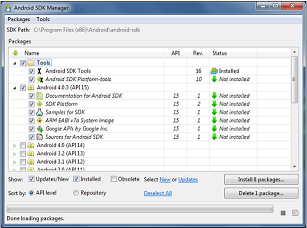
\includegraphics{Packages}
			\caption{Paquetes en SDK Manager}
			\label{fig:SdkManagerPackages}
		\end{figure}
		
	\newpage %Necesario para que la imagen aparezca antes de Firebase
	\subsection{Firebase}
		\begin{itemize}
			\item {\bf Librería}: Añadir la librería de Firebase en el archivo {\it ``build.gradle''} que esta dentro de la carpeta {\it ``app''} en el directorio raíz del proyecto.
				\lstinputlisting[float,language=Java,caption={Importación de la librería de {\it Firebase}},label={code:gradle}]{Code/build.gradle}
				
			\newpage
			\item {\bf Uso}: En los archivos de clase {\it ``java''}\cite{14:java:online} seguir los siguientes pasos:
				\begin{itemize}
					\item {\bf Librerías}: Se han de importar la librerías necesarias:
						\begin{itemize}
							\item {\bf Cliente Firebase}: Importar la librería del cliente.
							\item {\bf Errores Firebase}: Importar la librería de errores en consultas.
							\item {\bf Datos Firebase}: Importar la librería que permite la devolución de datos desde Firebase.
							\item {\bf Consultas Firebase}: Importar la librería para consultas.
							\item {\bf Librería Oyentes}: Importar la librería de los oyentes ({\it ``Listeners''}).
						\end{itemize}
					\item {\bf Contexto}: Añadir el contexto en que se va a usar en la función {\it onCreate}.
					\item {\bf Referencias}: Añadir una referencia a la base de datos o tabla de la misma a la que se van a hacer las consultas.
					\item {\bf Consultas}: Preparar la consulta que se va a hacer.
					\item {\bf Oyentes}: Añadir un oyente ({\it ``Listener''}) a la consulta.
				\end{itemize}
		\end{itemize}
		
		\lstinputlisting[float,language=Java,caption={Ejemplo de uso de {\it Firebase}},label={code:firebase}]{Code/FirebaseExample.java}
		
\newpage		
\section{Tutoriales}
	Antes de comenzar con el desarrollo de la aplicación, se han implementado varios tutoriales para afianzar los conocimientos sobre Android.
	\begin{enumerate}
		\item {\it Build your first app}\cite{29:firstapp:online} %En orden a partir de aquí
		\item {\it Adding the action bar}\cite{30:actionbar:online}
		\item {\it Supporting Different Devices}\cite{31:diferentdevices:online}
		\item {\it Managing the Activity Lifecycle}\cite{32:lifecycle:online}
		\item {\it Building a Dynamic UI with Fragments}\cite{33:fragments:online}
		\item {\it Saving Data}\cite{34:savingdata:online}
		\item {\it Interacting with Other Apps}\cite{35:interacting:online}
		\item {\it Sharing Simple Data}\cite{36:sharingsimpledata:online}
		\item {\it Sharing Files}\cite{37:sharingfiles:online}
		\item {\it Sharing Files with NFC}\cite{38:nfc:online}
		\item {\it Managing Audio Playback}\cite{39:audio:online}
		\item {\it Capturing Photos}\cite{40:photos:online}
		\item {\it Printing Content}\cite{41:printing:online}
		\item {\it Displaying Bitmaps Efficiently}\cite{42:bitmaps:online}
		\item {\it Displaying Graphics with OpenGL ES}\cite{43:opengl:online}
		\item {\it Animating Views Using Scenes and Transitions}\cite{44:transitions:online}
		\item {\it Adding Animations}\cite{45:animations:online}
		\item {\it Connecting Devices Wirelessly}\cite{46:connecting:online}
		\item {\it Performing Network Operations}\cite{47:networks:online}
		\item {\it Syncing to the Cloud}\cite{48:cloud:online}
		\item {\it Transferring Data Using Sync Adapters}\cite{49:adapters:online}
		\item {\it Best Practices for Security \& Privacy}\cite{50:securityprivacity:online}
		\item {\it Best Practices for Testing}\cite{51:testing:online}
		\item {\it Parse}\cite{52:parse:online}
		\item {\it Firebase Storage}\cite{53:firebase:online}
		\item {\it Expandable ListView}\cite{54:expandable:online}
		\item {\it TabHost Swipe}\cite{55:tabhostswipe:online}
		\item {\it ActionBar Tab Swipe}\cite{56:actionbartab:online}
	\end{enumerate} %Listo
	%
% ---------------------------------------------------
%
% Trabajo de Final de Grado:
% Author: Gonzalo Jesús García Martín <dracoyue@gmail.com>
% Capítulo: Especificación de Requisitos
% Fichero: Cap2_EspecificacionRequisitos.tex
%
% ----------------------------------------------------
%

\cleardoublepage
\chapter{Especificación de Requisitos}
\label{chap:requirements}

	\section{Funcionalidades}
		A continuación se describen las funcionalidades de la aplicación:
		\begin{itemize} 
			\item {\bf Registro}: Tras rellenar el formulario y accionar el botón de registro, \CollegeApp enviará los datos a la Firebase. Éstos serán almacenados en la base de datos, en sus tablas correspondientes. También creará al usuario correspondiente para que tenga acceso a la aplicación.
			\item {\bf Acceso}: El usuario introducirá su dirección de correo electrónico y contraseña en los campos destinados a ello. El dispositivo móvil se autenticará contra el servicio de Firebase y si todo es correcto permitirá el acceso.
			\item {\bf Recuerdo de Contraseña}: La aplicación solicitará al servicio en la nube una contraseña temporal para que el usuario pueda acceder, tras lo cual tendrá que editar su contraseña en \CollegeApp.
			\item {\bf Contactos}: Se recuperarán todos los usuarios relacionados con la persona que esté usando la aplicación. Esto permitirá que se puedan comunicar.
			\item {\bf chat}: Los usuarios se podrán enviar mensajes entre sí, éstos se almacenaran en Firebase para ser recuperados por la aplicación y luego borrados de la nube. La comunicación será del tipo alumno-profesor, padre-profesor y viceversa.
			\item {\bf Notificaciones}: \CollegeApp recuperará de la base de datos todos los mensajes que tenga el usuario, para después borrarlos de su almacenamiento en la nube.
			\item {\bf Circulares}: Aviso que mandará un profesor a todos los integrantes de una clase, e incluso de varias. Estos mensajes se almacenarán en la nube y serán recuperados por la aplicación, que los eliminará de su almacenamiento en internet.
			\item {\bf Citas}: Una vez concertada una cita con un profesor, se podrá mandar al calendario de Google para tenerla registrada.
			\item {\bf Visualización de Datos}: El usuario podrá visualizar la información de sus contactos con una selección larga en uno de ellos.
			\item {\bf Edición de datos}: Se podrá editar los datos en el dispositivo móvil, tras lo cual se actualizarán en la base de datos almacenada en la nube. 
		\end{itemize}

	%\section{Pantallas}
	\section{Actividades}
		La aplicación tendrá una pantalla de bienvenida con tres pestañas:
		\begin{itemize}
			\item Bienvenido: Aquí se mostrará los botones para acceder a la aplicación y para el registro de usuarios.
			\item Ayuda: En esta pestaña se obtendrá una pequeña ayuda sobre la aplicación.
			\item Sobre el Autor: Se mostrará la información sobre el autor de la aplicación.
		\end{itemize}
		
		En la pantalla de registro se le pedirá al usuario una serie de datos a cumplimentar según su rol: 
		\begin{itemize}
			\item Alumno:
				\begin{itemize}
					\item Nombre.
					\item Apellidos.
					\item Teléfono.
					\item Centro Escolar.
					\item Grupo y Curso al que pertenece: 1A, 2C, 3B... Solo podrá poner un curso y un grupo.
					\item Correo electrónico.
					\item Contraseña.
				\end{itemize}
			\item Profesor:
				\begin{itemize}
					\item Nombre.
					\item Apellidos.
					\item Teléfono.
					\item Centro Escolar.
					\item Grupo y Curso al que pertenece: 1A, 2C, 3B... Podrá poner varios cursos y grupos separados por comas.
					\item Correo electrónico.
					\item Contraseña.
				\end{itemize}
			\item Padre/Madre/Tutor Legal:
				\begin{itemize}
					\item Nombre.
					\item Apellidos.
					\item Teléfono.
					\item Centro Escolar al que asiste el alumno del que es padre.
					\item Correo electrónico.
					\item Contraseña.
					\item Nombre del alumno del que es padre.
					\item Apellidos del alumno del que es padre.
					\item Correo electrónico del alumno del que es padre.
					\item Centro escolar del alumno del que es padre.
					\item Curso y grupo del alumno del que es padre 1A, 2C, 3B... Solo podrá poner un curso y un grupo.
				\end{itemize}
		\end{itemize}
		
		En la pantalla de acceso se le pedirá su dirección de correo y la contraseña, el usuario tendrá, además, la posibilidad de solicitar que se le recuerde la contraseña por correo.
		
		\bigskip
		Una vez se accede a la aplicación a través del correo electrónico y contraseña, ésta se encarga de clasificar al usuario según el rol con el que se haya registrado, rellenando los datos de forma correcta según el perfil seleccionado. A continuación se describirá cada una de las pestañas en sus respectivos roles:
		\bigskip
		\begin{itemize}
			\item Alumnos:
				\begin{itemize}
					\item Alumnos: Esta pestaña contendrá los datos de los compañeros de clase del usuario.
					\item Profesores: Ésta se rellenará con los datos de los profesores que le dan clase al alumno.
					\item Notificaciones: En ésta se podrán encontrar los nombres de quienes envíen mensajes al usuario.
				\end{itemize}
			\item Profesores:
				\begin{itemize}
					\item Profesores: Aquí podremos encontrar los compañeros que dan clase a los grupos a los que el usuario da clase.
					\item Padres: Esta pestaña se rellenará con los padres de los alumnos a los que el profesor da clase.
					\item Alumnos: Aquí podremos encontrar a los alumnos a los que el profesor da clase
					\item Notificaciones: En ésta se podrán encontrar los nombres de quienes envíen mensajes al usuario.
				\end{itemize}
			\item Padres:
				\begin{itemize}
					\item Padres: En esta pestaña se encontrarán los padres de los compañeros de clase del hijo/s del usuario.
					\item Profesores: Aquí estarán los profesores que dan clase al hijo/s del usuario.
					\item Notificaciones: En ésta se podrán encontrar los nombres de quienes envíen mensajes al usuario.
				\end{itemize}
		\end{itemize}
										
		Los profesores tendrán una opción para enviar circulares a otros usuarios de la aplicación. Los padres podrán concertar citas con los profesores y viceversa.
		Al seleccionar cualquiera de los usuarios que aparecen en las listas, se lanzará un ``chat'' para que los usuarios se comuniquen entre ellos. Al enviar un mensaje éste se almacenará en los servicios en la nube, en la tabla destinada a los mensajes. Esta tabla contendrá el mensaje, el destinatario y el remitente. Cuando el dispositivo reciba el mensaje, lo borrará de la tabla para no sobrecargarla.
		
		\bigskip
		Al hacer una selección larga, se podrán ver los datos del usuario que se selecciona.
	
		Todos los datos estarán almacenados en la nube, en concreto en los servicios de Firebase\cite{6:firebase:online} que es propiedad de Google\cite{18:google:online}.

	\section{Sistemas de la Aplicación}
		\begin{itemize}
			\item Sistema de Registro: Al usuario se le podrá pedir los siguientes datos, según el rol con el que se registre:
			\begin{itemize}
				\item Nombre y Apellidos.
				\item Rol con el que se va a registrar, ya que en función de un rol u otro se le pedirá distintos datos.
				\item Número de teléfono.
				\item Nombre del centro con el que va a hacer el registro.
				\item Clase y grupo.
				\item E-mail y contraseña.
				\item Nombre y Apellidos del alumno.
				\item Clase en la que está el alumno.
				\item Centro en el que está el alumno.
				\item Curso en el que está el alumno.
			\end{itemize}
			\item Sistema de ``acceso'': Se le pedirá al usuario que ingrese su identificación, es decir, su e-mail y contraseña.
			\item Sistema de comunicación entre alumnos, profesores y padres/madres/tutores legales: Tanto los profesores como los padres/madres/tutores legales se podrán comunicar entre sí con un servicio tipo ``chat'', para informar de alguna incidencia, mensaje o notificación. Este servicio enviará los mensajes a través de internet usando los servicios de ``firebase''.
			\item Sistema de citas: Se podrá concertar citas con los padres/madres/Tutores Legales, así como éstos podrán solicitar reuniones con los profesores, estas citas se podrán añadir al calendario de Google.
			\item Lista de contactos, organizada por grupos desplegables, por ejemplo los profesores tendrán la lista organizadas por las clases que impartan en el centro.
		\end{itemize}
	
		Esto permitirá establecer un sistema de comunicaciones entre los profesores y los padres de alumnos.

	\section{Roles}
		\begin{itemize}
			\item Alumnos: Se podrá comunicar con los profesores, pudiendo solicitar citas y recibir circulares.
			\item Profesores: Se podrá comunicar con los alumnos y padres, pudiendo solicitar citas y enviar circulares. Los padres y alumnos en la lista de contactos estarán organizados por las clases que impartan en el centro.
			\item Padre/Madre/Tutor Legal: Se podrá comunicar con los profesores, pudiendo recibir circulares y solicitar citas. Los profesores en la lista de contactos estarán organizados las clases que impartan a los alumnos con los que el progenitor esté relacionado.
		\end{itemize}
 %Listo
	%
% ---------------------------------------------------
%
% Trabajo de Final de Grado:
% Author: Gonzalo Jesús García Martín <dracoyue@gmail.com>
% Capítulo: Objetivos
% Fichero: Cap3_Objetivos.tex
%
% ----------------------------------------------------
%

\cleardoublepage
\chapter{Objetivos}
\label{chap:objetives}

	En este capítulo se pasará a describir tanto los objetivos generales como los específicos.
	
	%%%%%%%%%%%%%%%%%%%%%%%%%%%%%%%%%%%%%%%%%%%%%%%%%%%%%%%%%%%%%%%%%%%%%%%%%%%%%%%%%%%%%%%%%%%%%%%%%%%%%
	%Objetivos generales:
	%
	%Los objetivos generales corresponden a las finalidades genéricas de un proyecto o entidad.
	%
	%No señalan resultados concretos ni directamente medibles por medio de indicadores pero si que expresan el propósito central del proyecto.
	%Tienen que ser coherentes con la misión de la entidad. 
	%%%%%%%%%%%%%%%%%%%%%%%%%%%%%%%%%%%%%%%%%%%%%%%%%%%%%%%%%%%%%%%%%%%%%%%%%%%%%%%%%%%%%%%%%%%%%%%%%%%%%
	\section{Objetivos Generales}
		Se pretende crear una aplicación en Android como trabajo de fin de grado, utilizando las nuevas tecnologías como los teléfonos inteligentes y los servicios gratuitos de internet conocidos como ``Nube''\cite{57:nube:online}.
	
	\section{Objetivos Específicos}
		%Objetivos específicos
		%
		%Se derivan de los objetivos generales y los concretan, señalando el camino que hay que seguir para conseguirlos. Indican los efectos
		%específicos que se quieren conseguir aunque no explicitan acciones directamente medibles mediante indicadores. 
		
	%
% ---------------------------------------------------
%
% Trabajo de Final de Grado:
% Author: Gonzalo Jesús García Martín <dracoyue@gmail.com>
% Capítulo: Objetivos
% Fichero: Cap4_Antecedentes.tex
%
% ----------------------------------------------------
%

\cleardoublepage
\chapter{Antecedentes}
\label{chap:record}

	Con los nuevos avances tecnológicos se ha vuelto popular el uso de las comúnmente denominada ``apps'' en los dispositivos móviles. Hay aplicaciones para todos los gustos, desde lo mas básico como aprender a cocinar o aplicaciones de comunicación, hasta de lo más importante como por ejemplo consultar la información de la cuenta del banco e incluso hacer operaciones con ella.
	
	\bigskip
	Se ha observado que en el ámbito docente hay una falta de comunicación entre padres y profesores. También el aumento de problemas como el acoso, fracaso escolar o incluso problemas de ámbito familiar influyen en los alumnos. Por eso los hasta ahora recursos tradicionales no eran suficientes. Notas escritas y reuniones no son mas que informes puntuales de un progreso continuo que puede decaer sin aviso previo.
	
	\bigskip
	Por eso se presenta una herramienta que intenta establecer un flujo de información continua sin comprometer los datos personales de los usuarios tales como el teléfono o el correo. Así éstos se sentirán cómodos a la hora de comunicarse de forma segura. Se entiende que es un esfuerzo extra para los equipos docentes, pero permitirá que haya una mejor comunicación para resolver problemas inesperados y actuar de forma casi inmediata. %Listo
	%
% ---------------------------------------------------
%
% Trabajo de Final de Grado:
% Author: Gonzalo Jesús García Martín <dracoyue@gmail.com>
% Capítulo: Objetivos
% Fichero: Cap5_Problemas.tex
%
% ----------------------------------------------------
%

\cleardoublepage
\chapter{Problemas}
\label{chap:troubles}

	\begin{enumerate}
		\item {\bf Android Studio no render target}
			\begin{itemize}
				\item {\em Solución}:
					\begin{enumerate}
						\item Asegurarse de que hay un dispositivo real o virtual seleccionado.
						\item Tener una versión de Android seleccionada.
						\item Versiones necesarias para el desarrollo dela aplicación en Android instaladas.
						\item Crear un nuevo Dispositivo Virtual (AVD).
						% Meter dibujo de AVD
						\item reiniciar Android Studio.
					\end{enumerate}
			\end{itemize}
		%
		\item {\bf Fallo al encontrar com.android.support:appcompat-v7:16.+}
			\begin{itemize}
				\item {\bf Solución}: Actualizar en las dependencias del archivo ``build.gradle'', en el directorio ``app'' que está en la raíz del proyecto, la librería a la última versión disponible de forma manual.
			\end{itemize}
		%
		\item {\bf Fallo al encontrar Java}
			\begin{itemize}
				\item {\bf Solución}: Si java ya está instalado, averiguar el directorio. Una vez echo esto necesitas volver a establecer la variable de ámbito indicando la localización correcta.
				Selecciona Iniciar \textgreater Equipo \textgreater Propiedades \textgreater Configuración Avanzada del Sistema.
				Entonces abre la pestaña Opciones Avanzadas \textgreater Variables de Entorno y añade una nueva variable de sistema llamada JAVA\_HOME que redirija a tu directorio JDK, por ejemplo ``C:{\textbackslash}Program Files{\textbackslash}Java{\textbackslash}jdk1.7.0\_21''. 
			\end{itemize}
		\item {\bf Duplicidad en las dependencias de los paquetes}
			\begin{itemize}
				\item {\bf Solución}: Si se tiene un error de construcción compilando sobre archivos duplicados, se puede excluir esos ficheros añadiendo la directiva {\it packagingOptions} al archivo {\it build.gradle} que está en el directorio {\it app}.
				
				\lstinputlisting[float,language=Java,caption={Solución a la duplicidad en build.gradle},label={code:duplicidadbuild}]{Code/duplicidadbuild.gradle}
			\end{itemize}
			
		\newpage
		\item {\bf Porblemas con import android.support.v13}
			\begin{itemize}
				\item {\bf Solución}: Añadir en las dependencias del archivo ``build.gradle'', en el directorio ``app'' que está en la raíz del proyecto, la orden ``compile 'com.android.support:support-v13:21.+' '' de forma manual.
				
				\noindent
				\lstinputlisting[float,language=Java,caption={Solución al problema supportV13},label={code:supportv13}]{Code/support13build.gradle}
			\end{itemize}
			
		\newpage
		\item {\bf Problemas con Gradle}
			\begin{itemize}
				\item {\bf Solución}:
					\begin{enumerate}
						\item En el archivo ``buil.gradle'' que está en el directorio raíz del proyecto añadir la dependencia de forma manual: {\it classpath 'com.android.tools.build:gradle:1.0.0'}.
						\item En el archivo ``buil.gradle'' que está en el directorio ``app'' en la raíz del proyecto añadir dentro de ``release'' de forma manual:
							minifyEnabled false\\
							proguardFiles getDefaultProguardFile('proguard-android.txt'), 'proguard-rules.txt'
					\end{enumerate}
					\noindent
					\lstinputlisting[float,language=Java,caption={Solución en build.gradle},label={code:buildGradle}]{Code/buildgradle.gradle}
					\lstinputlisting[float,language=Java,caption={Solución en app/build.gradle},label={code:appBuildGradle}]{Code/appbuildgradle.gradle}
			\end{itemize}
		
		\newpage
		\item {\bf SDK no encontrado}
			\begin{itemize}
				\item {\bf Solución}: Si Android Studio no encuentra el SDK y está instalado seleccionar {\it Windows \textgreater Preferencias \textgreater Android \textgreater Localización SDK} y establecer el directorio donde se tiene instalado.
			\end{itemize}
			
		\item {\bf Consultas Asíncronas}
			\begin{itemize}
				\item {\bf Solución}: Existen dos tipos de consultas en Firebase, las que devuelven un solo resultado (``{\it addListenerForSingleValueEvent}'') y las que devuelven varios resultados (``{\it addChildEventListener}''). Éstas últimas se quedan esperando por si se modifican datos de la base de datos.
				La solución sería removerlo al final de su uso (``{\it ref.removeEventListener(originalListener);}'') o tener una sola consulta del segundo tipo por actividad.
			\end{itemize}
	\end{enumerate} %Listo
	%
% ---------------------------------------------------
%
% Trabajo de Final de Grado:
% Author: Gonzalo Jesús García Martín <dracoyue@gmail.com>
% Capítulo: Fases
% Fichero: Cap6_Fases.tex
%
% ----------------------------------------------------
%

\cleardoublepage
\chapter{Fases}
\label{chap:phases}

	Las fases de diseño del proyecto fueron las siguientes:
	
%	\begin{enumerate}
%		\item Identificar las funcionalidades de la aplicación, es decir, la especificación de requisitos.
%		\item Escoger una funcionalidad concreta.
%		\item Implementar esa parte de la aplicación.
%		\item Probar el código resultante y corregir los errores que pueda ocasionar.
%		\item Corrección de errores y adaptación de otras partes de la aplicación para la correcta integración de la nueva funcionalidad.
%		\item Si se encuentra una nueva funcionalidad añadirla a las ya identificadas.		
%		\item se seguirán estas indicaciones hasta haber implementado todos los requisitos de la aplicación.
%	\end{enumerate}

	\bigskip
	Primero se identifican las funcionalidades de la aplicación, es decir, la especificación de requisitos. Se escoge un requisito concreto de los que han sido identificados, se implementa la parte de la aplicación que corresponde con la funcionalidad escogida. Se prueba el código resultante y se corrigen los errores que puedan surgir en esta implementación, también se adaptan partes del código para que trabajen en conjunto con la nueva funcionalidad y se vuelve a la corrección de errores que puedan surgir. Por último se escoge otro requisito que implementar. Si se encuentra un nuevo requisito o funcionalidad que deba ser programado, se añadirá a las ya existentes.
	
	\bigskip
	Se siguen estas indicaciones hasta que la aplicación esté completa, es decir, hasta que no queden requisitos que sin cumplir. %Listo
	%
% ---------------------------------------------------
%
% Trabajo de Final de Grado:
% Author: Gonzalo Jesús García Martín <dracoyue@gmail.com>
% Capítulo: Desarrollo del Proyecto
% Fichero: Cap7_DesarrolloProyecto.tex
%
% ----------------------------------------------------
%

\cleardoublepage
\chapter{Desarrollo del Proyecto}
\label{chap:developing}

	Se toma contacto con las herramientas a utilizar. Para afianzar y adquirir conocimientos nuevos se implementan diferentes tutoriales orientados a facilitar la ejecución correcta del proyecto. Se especifican los requisitos de la aplicación y se deciden los servicios en la nube que se van a usar.
	Se usa UML\cite{58:UML:online} para crear el diagrama de actividades y flujo; se buscan aplicaciones similares y se implementa una base de datos en los servicios web elegidos. Se crean las actividades básicas de la aplicación para conseguir registro y autenticación de usuarios, además de decir el estilo que tendrá la aplicación.
	
	\bigskip
	Se implementa la actividad donde se mostrarán los contactos de usuario. Pero hay un problema con las consultas y es que son asíncronas, es decir, el código se sigue ejecutando mientras la consulta no ha terminado.
	Introducimos mas usuarios en nuestra base de datos y le añadimos a la aplicación cierta navegabilidad. También se crea la función que comprueba si el dispositivo tiene internet y la encargada de comprobar si un alumno existe cuando un usuario con el perfil de padre se registra. Se adapta el registro para incluir los diferentes perfiles de los usuarios que van a usar la aplicación.
	
	\bigskip
	Se ponen todos los botones en español, se programa el código que recupera las notificaciones de un usuario y se gestionan los colegios desde la base de datos añadiendo información de éstos. Se comprueban los campos en los que el usuario tiene que introducir datos, además de codificar la diferenciación de las notificaciones según el perfil del usuario remitente y se usa una imagen para mostrar los campos obligatorios.
	
	\bigskip
	Se implementan las actividades de ayuda, la que se usa para programar eventos en el calendario y la que usarán los usuarios con perfil de profesor para enviar una notificación a los integrantes de una misma clase, ya sean usuarios con el perfil de padre o con el de alumno. Se añaden los idiomas de inglés y francés, se resuelven los problemas que se derivan de éstos pues al cambiar la orientación del dispositivo,  se recreaba la actividad con el lenguaje por defecto del dispositivo. Esto se solucionó almacenando el idioma seleccionado y recuperándolo al inicio de cada actividad.
	
	\bigskip
	Se gestionan las clases de cada colegio desde la base de datos añadiendo información sobre éstas y se cambia la recuperación de usuarios desde dicha base. Se recuperaban atendiendo al correo de los usuarios, pero como los usuarios con perfil de alumno registrados por otro que tenga un perfil de padre pueden no tener correo, se usa el DNI. Por último se añade la funcionalidad para contraseñas olvidadas, dar de baja una cuenta y salir de la aplicación. %Listo
	%
% ---------------------------------------------------
%
% Trabajo de Final de Grado:
% Author: Gonzalo Jesús García Martín <dracoyue@gmail.com>
% Capítulo: Fases
% Fichero: Cap8_Conclusiones_LineasFuturas.tex
%
% ----------------------------------------------------
%

\cleardoublepage
\chapter{Conclusiones y Lineas futuras}
\label{chap:conclusions}

	\section{Lineas futuras}
		Se contemplarán casos de uso que no se han contemplado a la hora de crear la aplicación. Perfiles como padres con hijos en distintos centros, profesores que trabajen en mas de un centro o usuarios con distintos perfiles en el mismo centro, por ejemplo, un profesor que de clases en el colegio al que asiste su hijo.
		
	\section{Conclusiones}
		La realización de este proyecto permite aplicar los conocimientos técnicos obtenidos durante los años de estudio permitiendo la asimilación real de las competencias necesarias y adquirir nuevos conocimientos.
		Esta experiencia da a conocer el grado de implicación que conlleva crear una aplicación totalmente funcional en un ámbito real. El análisis de otras aplicaciones similares permite concretar el estado del mercado con respecto al tipo de aplicación creada.
		
		\bigskip
		Programar una aplicación puede parecer sencillo, pero conlleva dedicación, tiempo, trabajo y esfuerzo. %Listo
	%
% ---------------------------------------------------
%
% Trabajo de Final de Grado:
% Author: Gonzalo Jesús García Martín <dracoyue@gmail.com>
% Capítulo: Fases
% Fichero: Cap9_Cap8English.tex
%
% ----------------------------------------------------
%

\cleardoublepage
\chapter{Conclusions and Future lines}
\label{chap:futureLines}

	\section{Future lines}
		Use cases that have not been contemplated when creating the application will be contemplated. Profiles as parents with children in different schools, teachers working in more than one center or users with different profiles on the same center, for example, a school teacher in the school that your child attends.
	
	\section{Conclusions}
		The realization of this project will apply the expertise gained during the years of study allowing real assimilation of the necessary skills and acquire new knowledge.
		This experience discloses the level of involvement that involves creating a fully functional application in a real environment. The analysis of other similar applications can realize the state of the market for the type of application built.
		
		\bigskip
		An application program may seem simple, but it takes dedication, time and hard work. %Listo
	%
% ---------------------------------------------------
%
% Trabajo de Final de Grado:
% Author: Gonzalo Jesús García Martín <dracoyue@gmail.com>
% Capítulo: Objetivos
% Fichero: Cap10_Presupuesto.tex
%
% ----------------------------------------------------
%

\cleardoublepage
\chapter{Presupuesto}
\label{chap:budget}

	Adquisición de 2 dispositivos de gama media: 2 x 119 euros = 238 euros.\\
	Mano de obra: 60 días de trabajo x 8 horas diarias = 480 horas de trabajo.\\
	480 horas de trabajo * 2,50 euros la hora = 1200 euros.\\
	Total : 1438 Euros. %Listo
	
%%%%%%%%%%%%%%%%%%%%%%%%%%%%%%%%%%%%%%%%%%%%%%%%%%%%%%%%%%%%%%%%%%%%%%%%%%%%%%%%%%%%%%%%%%%%%%%%
%%%%%%Apéndices%%%%%%
	\appendix
	%\appendixname
	%
% ---------------------------------------------------
%
% Trabajo de Final de Grado:
% Author: Gonzalo Jesús García Martín <dracoyue@gmail.com>
% Capítulo:  diagrama de Clases
% Fichero: ApendiceA_diagramaClases.tex
%
% ----------------------------------------------------
%

\cleardoublepage
\chapter{Diagrama de Clases}
\label{chap:classdiagram}

Se puede ver una imagen del diagrama de clases:

\begin{figure}[h !]
	\centering
	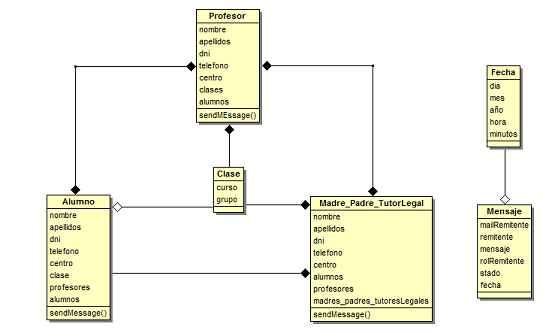
\includegraphics{CollegeAppDiagramaClases}
	\caption{Diagrama de Clases}
	\label{fig:ClassDiagram}
\end{figure}
 %Listo
	%
% ---------------------------------------------------
%
% Trabajo de Final de Grado:
% Author: Gonzalo Jesús García Martín <dracoyue@gmail.com>
% Capítulo:  Diagrama de actividades
% Fichero: ApendiceB_DiagramaActividades.tex
%
% ----------------------------------------------------
%

\cleardoublepage
\chapter{Diagrama de Actividades}
\label{chap:activitiesdiagram}

Se puede ver una imagen del diagrama de actividades:

\begin{figure}[h !]
	\centering
	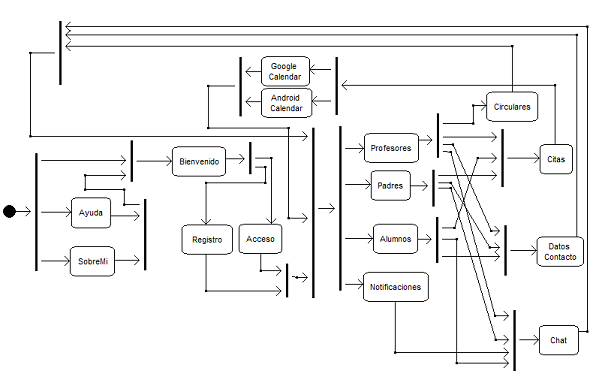
\includegraphics{CollegeAppDiagramaActividades}
	\caption{Diagrama de Actividades}
	\label{fig:ActivitiesDiagram}
\end{figure}

Cada uno de los nodos es una actividad, representando las flechas el acceso a otras actividades. Las barras verticales representan que desde múltiples actividades se pueden acceder a una o varias. %Listo
	%
% ---------------------------------------------------
%
% Trabajo de Final de Grado:
% Author: Gonzalo Jesús García Martín <dracoyue@gmail.com>
% Capítulo:  Diagrama de actividades
% Fichero: ApendiceC_MapaActividades.tex
%
% ----------------------------------------------------
%

\cleardoublepage
\chapter{Secuencia de Actividades}
\label{chap:activitiesSecuence}

Se puede ver una imagen de la secuencia de actividades que sigue la aplicación:

\begin{figure}[h]
	\centering
	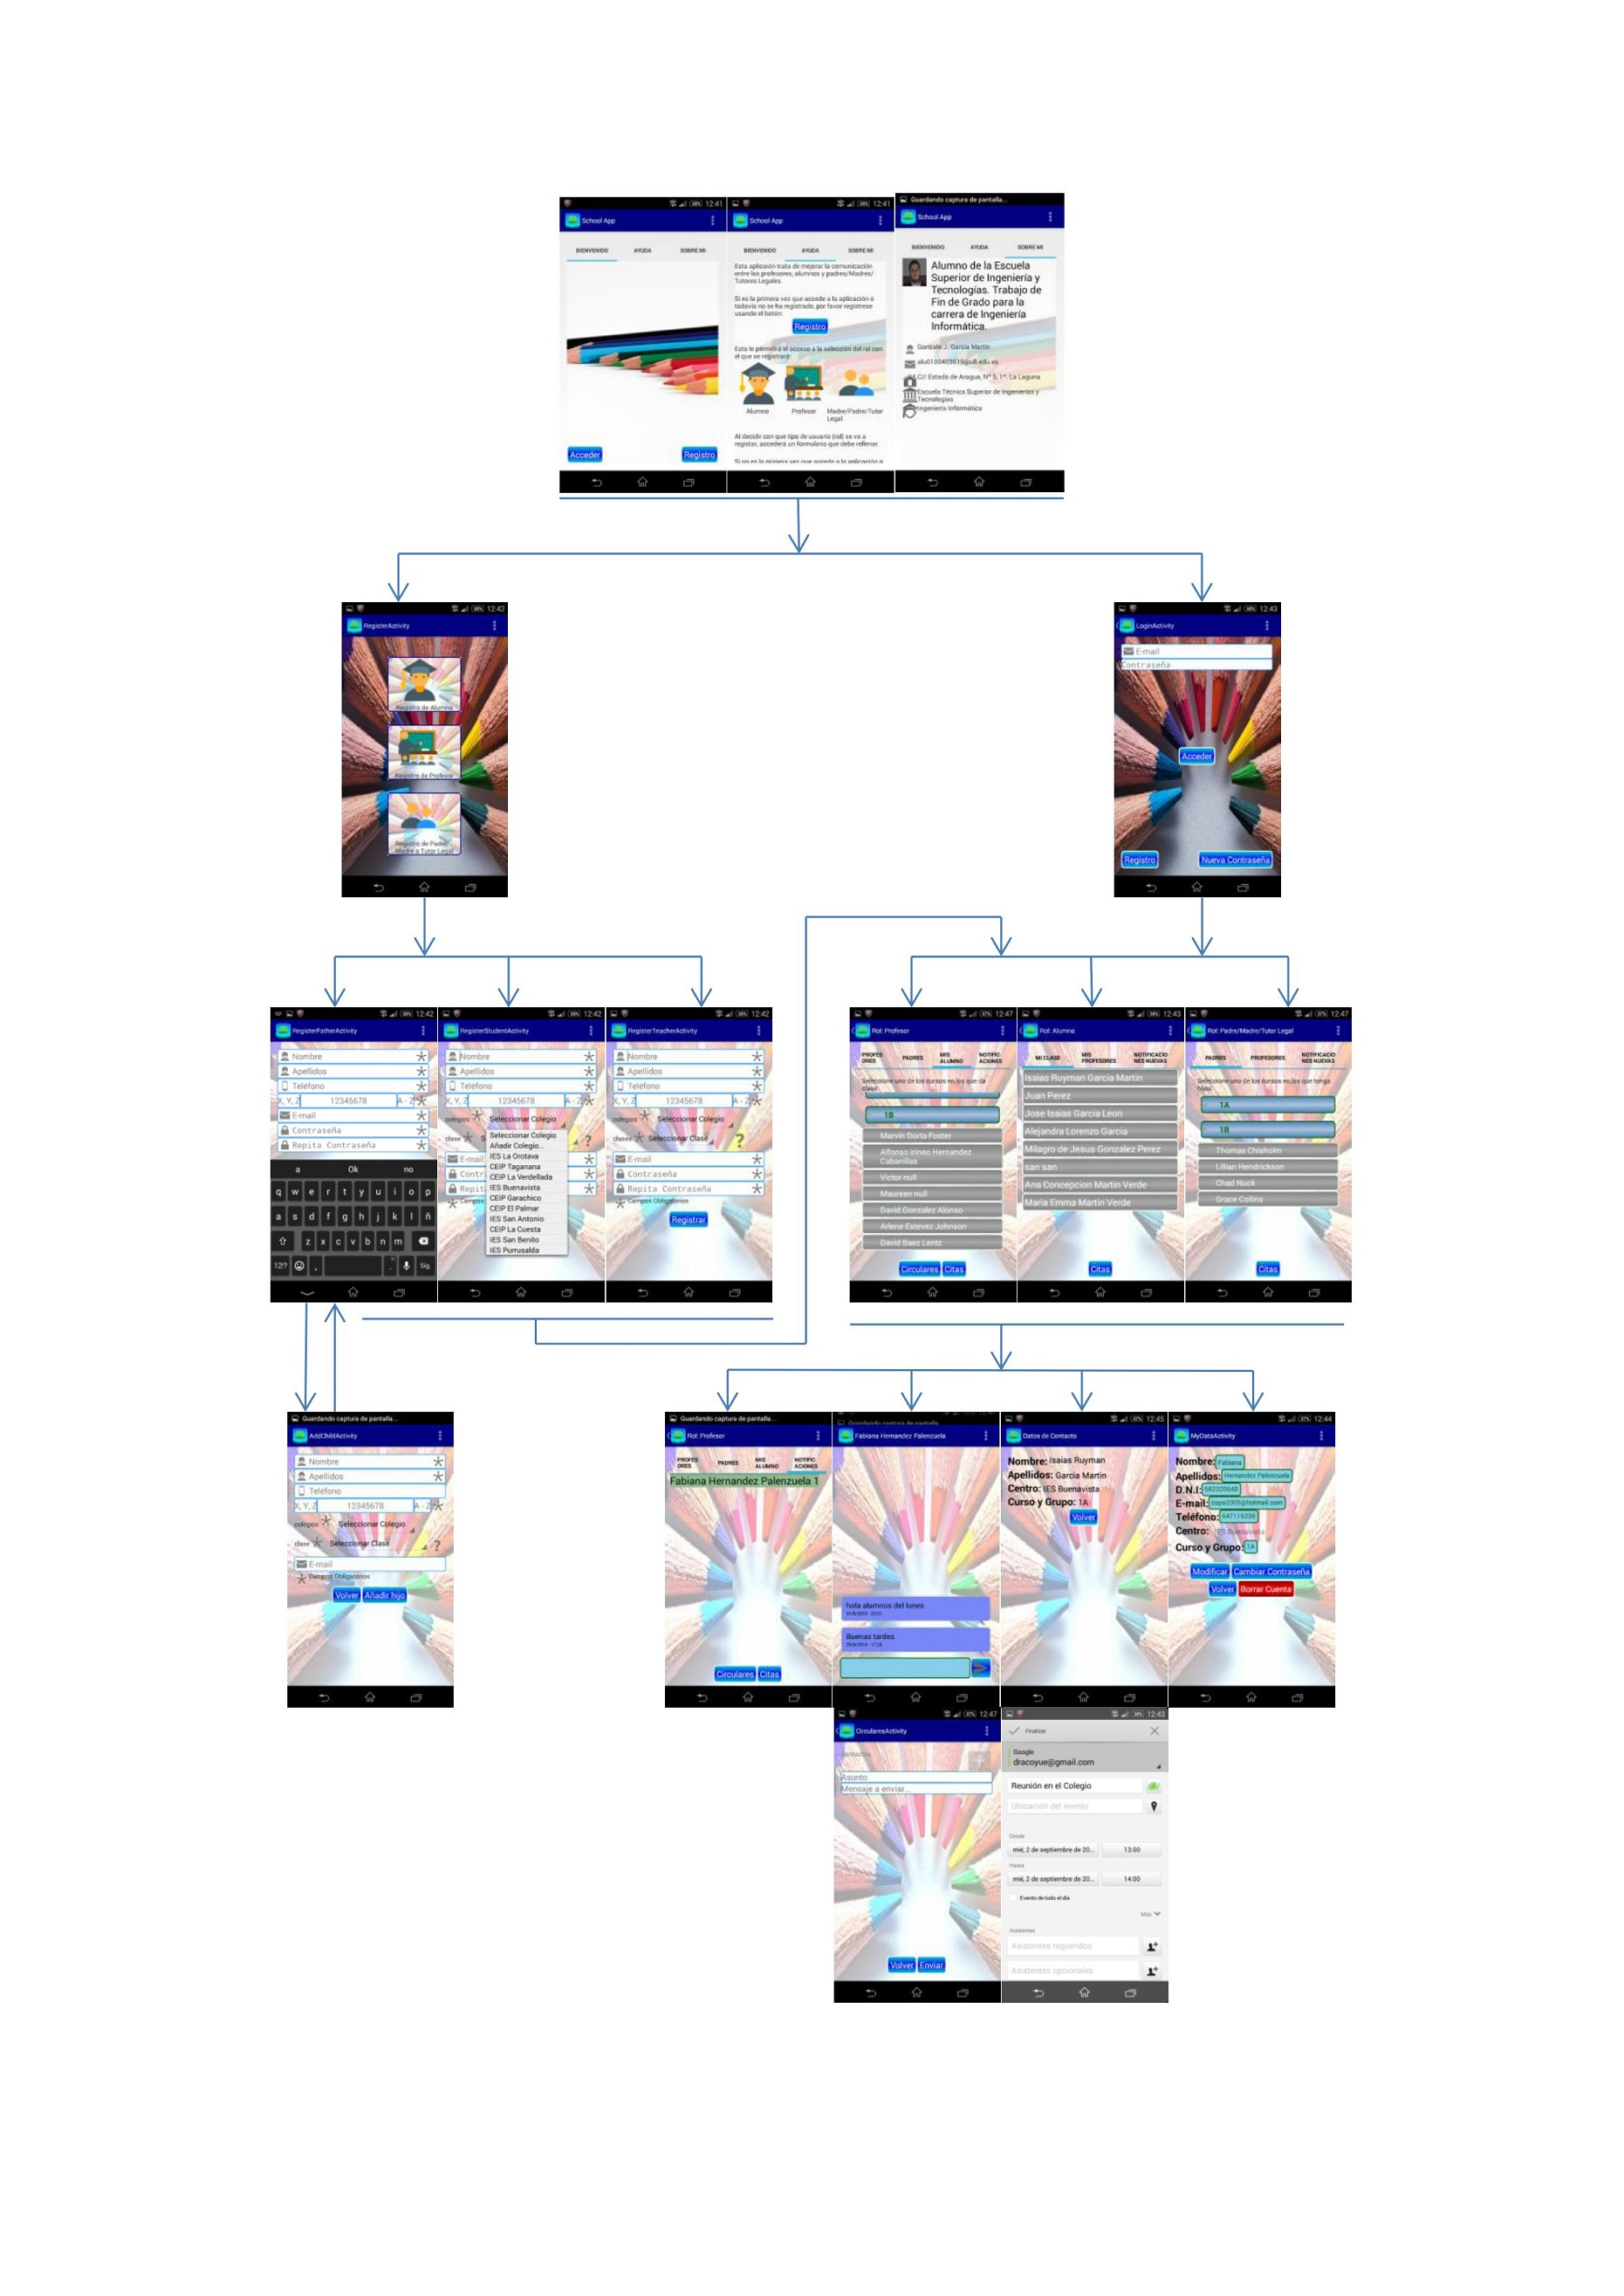
\includegraphics{mapaActividades}
	\caption{Secuencia de Actividades}
	\label{fig:ActivitiesSecuence}
\end{figure} %Listo
	
%%%%%%%%%%%%%%%%%%%%%%%%%%%%%%%%%%%%%%%%%%%%%%%%%%%%%%%%%%%%%%%%%%%%%%%%%%%%%%%%%%%%%%%%%%%%%%%%
	%Bibliografía
	\bibliographystyle{unsrt}
	\bibliography{Bibliografia/bibliography}
	
\end{document}
